\documentclass[5pt]{standalone}

\usepackage{tikz}
\usetikzlibrary{calc}

\usepackage{physics}

\begin{document}
	
	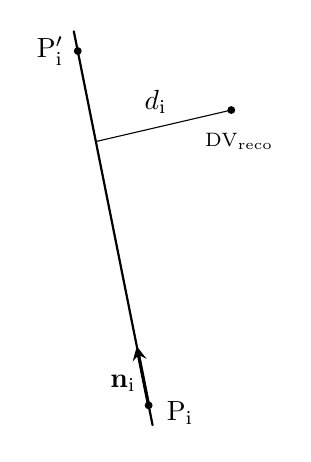
\begin{tikzpicture}[line cap = round]
%		% Grid
%		\draw (0,0) grid (5,5);
%		\foreach \i in {0,1,...,5}
%		{
%			\node at (-1ex, \i) {\i};
%			\node at (\i, -1ex) {\i};
%		}
		
		% Coordinates
		\coordinate (A) at (1,0);
		\coordinate (B) at (0,5);
		\coordinate (P1) at ($(A)!0.05!(B)$);
		\coordinate (P2) at ($(A)!0.95!(B)$);
		\coordinate (P3) at ($(A)!0.2!(B)$);
		\coordinate (P3') at ($(P3)!0.5!(P1)$);
		\coordinate (P4) at ($(A)!0.72!(B)$);
		\coordinate (DVreco) at (2,4);
		\coordinate (DV-P4) at ($(DVreco)!0.5!(P4)$);
		
		% Lines
		\draw[thick] (A) -- (B);
		\draw[] (DVreco) -- (P4);
		\draw[very thick, -stealth] (P1) -- (P3);
		
		% Points
		\draw[fill=black, draw=black] (P1) circle (1.2pt);
		\draw[fill=black, draw=black] (P2) circle (1.2pt);
		\draw[fill=black, draw=black] (DVreco) circle (1.2pt);
		
		% Nodes
		\node[shift={(0.1,-0.4)}] at (DVreco) {\scriptsize$\mathrm{DV}_\mathrm{reco}$};
		\node[shift={(0.4,-0.1)}] at (P1) {$\mathrm{P}_\mathrm{i}$};
		\node[shift={(-0.35,0)}] at (P2) {$\mathrm{P}'_\mathrm{i}$};
		\node[shift={(-0.1,0.3)}] at (DV-P4) {$d_\mathrm{i}$};
		\node[shift={(-0.25,-0.1)}] at (P3') {$\vb{n}_\mathrm{i}$};
	\end{tikzpicture}
	
\end{document}